\documentclass{article}

% Packages are like plug-ins that add functionality
\usepackage{amsthm, amssymb, amsmath} % basic math stuff -- always include this
\usepackage[colorlinks=true]{hyperref} % clickable hyperlinks
\usepackage{enumitem} % customize enumeration 
\usepackage[margin=1in]{geometry} % adjust margins

\usepackage[all]{xy} % xymatrix and xypic
\usepackage{tikz} % tikz for drawing graphs and pictures
% \setlength\parindent{0em} % never indent a paragraph

\usepackage{booktabs} % for tables
\usepackage[normalem]{ulem}
\useunder{\uline}{\ul}{}

\usepackage[backend=biber]{biblatex} % references
\addbibresource{refs.bib}


% graphics
\usepackage{graphicx} % include images
\graphicspath{ {./figures/} }

% This sets up macros (short forms) for common commands
\newcommand{\R}{\mathbb{R}} % This sets up the command \R and it writes that funny R that we use to designate R^2 and R^3

% Here is where the main content starts
\begin{document}

% This sets up the title and author
\title{Introduction to the \textbf{Experimental and Computational Analyses of Viscous Droplet Motion through Straight Microchannels} project}
\author{\large Ashish Srivastava $\vert$ CHEN 4010 – Senior Thesis}
\date{\today} % this will typeset the date of typesetting
\maketitle

\mbox{}
\vfill

\begin{center}
\large
Dr. Carolyn Kohlmeier \\
Instructor \\
Department of Chemical and Biological Engineering \\
University of Colorado Boulder
\end{center}

\begin{center}
\large
Dr. Robert Davis \\
Tisone Professor and Dean Emeritus \\
Department of Chemical and Biological Engineering \\
University of Colorado Boulder 
\end{center}

\pagebreak

% \section{Introduction}

\section{Goal of the Project} \label{goals}

This project aims to better characterize the behavior of viscous microdroplets moving through straight, rectangular microchannels. Namely, the project will focus on quantifying the steady-state velocity and deformation of the droplets as a result of changing different parameters of the flow (specifically the viscosity ratio $\lambda$ between the droplet and bulk fluid, the Capillary number $Ca$, the Reynolds number $Re$, and the geometry of the rectangular channel). The project will be two-fold (potentially three-fold): the simulation portion of the investigation will utilize the numerical Boundary-Integral method to simulate the droplets, and a macroscopic flow-cell will be used to validate the results from our simulation. Circumstances allowing, the project may be extended to employ facilities in the Mechanical Engineering department to conduct experiments at the traditional microfluidic scale using a PDMS flow-chip. 

\section{Significance and Broader Impacts}

Microfluidic systems have become prevalent throughout several technical applications in recent years. Microfluidic phenomena are being leveraged in applications for systems such as drug delivery, single-cell assays, microfluidic biochemical synthesis, and medical devices \cite{theberge_microdroplets_2010}. Microdroplets specifically lend scientists and engineers the ability to manipulate small controllable volumes for performing reactions or studying single cells thus making them ideal for high-throughput experimentation \cite{sackmann_present_2014}. 
Within all of these applications, the individual branches of many microfluidic systems consist of straight rectangular channels and it is important to be able to control and predict parameters such as droplet path, deformation, and breakup. Thus, it is imperative to be able to characterize how physical and geometric parameters affect the motion of droplets travelling through these channels. Being able to predict droplet behavior is not a trivial undertaking, and scale microfluidic chips are not easy to manufacture (specialized equipment for processes such as plasma cleaning and photolithography are necessary). 

The results from this investigation will allow for improved, more-informed design of microfluidic systems. If the macroscopic flow cell is shown to accurately model microfluidic phenomena it will mean that specialized equipment is not strictly necessary for the prototyping of microfluidic designs, making microfluidic research more accessible to investigators. Additionally, by characterizing droplet behavior as a function of fluid parameters, the results of this study can aid in quantifying deformable droplet stability as drops travel down the length of microfluidic channels. 

\section{Prior Research}
The Davis group at the University of Colorado Boulder has undertaken several studies related to the dynamics of microdroplets flowing through microchannels. Zinchenko et. al. developed a three-dimensional Boundary-Integral algorithm in Fortran to simulate viscous droplets within a low $Re$ regime \cite{zinchenko_novel_1997}. This algorithm was further developed by Navarro et. al. \cite{rociophd_thesis} for the case of a droplet moving through finite-depth channels (as opposed to the previous work done for infinite-depth simulations). 

The group has also performed a range of simulations where the viscosity ratio $\lambda$, dimensionless drop size $d/H$, capillary number $Ca$, and aspect ratio $W/H$ were altered and the velocity of the droplet was recorded as a time series. Previous work I did with the group tabulated the steady-state velocity of droplets under different conditions, and I aim to expand on this work to the lower limit of conditions allowable by the Boundary-Integral code. 

Additional work by Navarro et. al. conducted with Professor Patrick Spicer at the University of South Wales observed deformable droplets in PDMS microfluidic chips and identified that shape manipulation of droplets could be attained simply with junctions and flow control \cite{rociophd_thesis}. The results from these experiments were compared with results from the Davis group's Boundary-Integral simulations, and good agreement was found between the two \cite{rociophd_thesis}. This project aims to expand on this work by comparing experimental and numerical simulation results specifically for the case of simple, straight channels. 

\section{Details of the Proposed Study}
As indicated in Section \ref{goals}, this project consists of several distinct but overlapping sub-projects: (\textbf{Aim 1}) is to collect experimental data from a macroscopic flow-cell apparatus, (\textbf{Aim 2}) is to run simulations with the same parameters as the experiments from Aim 1, and a potential extension is (\textbf{Aim 3}) which would investigate the same flow setup but at the scale of a microfluidic chip rather than the macroscopic cell in Aim 1.

In \textbf{Aim 1}, we are using a macroscopic flow cell for ease of visualization of the microdroplets' behavior. We have identified fluid systems (for both the droplet and bulk fluids) where the density of the fluids is comparable (as to avoid any gravitational settling effects as the droplet travels down the length of the flow cell). Our current setup is using castor oil ($\rho_{oil} = 1.018 g/mL$) as the bulk fluid, then adjusting the droplet fluid. We have used both polydimethylsiloxane (PDMS, a silicone oil) and a glycerol/water mixture to produce droplets of different viscosities, but comparable densities to the bulk castor oil. Below is an image of the CAD design of the flow cell:
\begin{center}
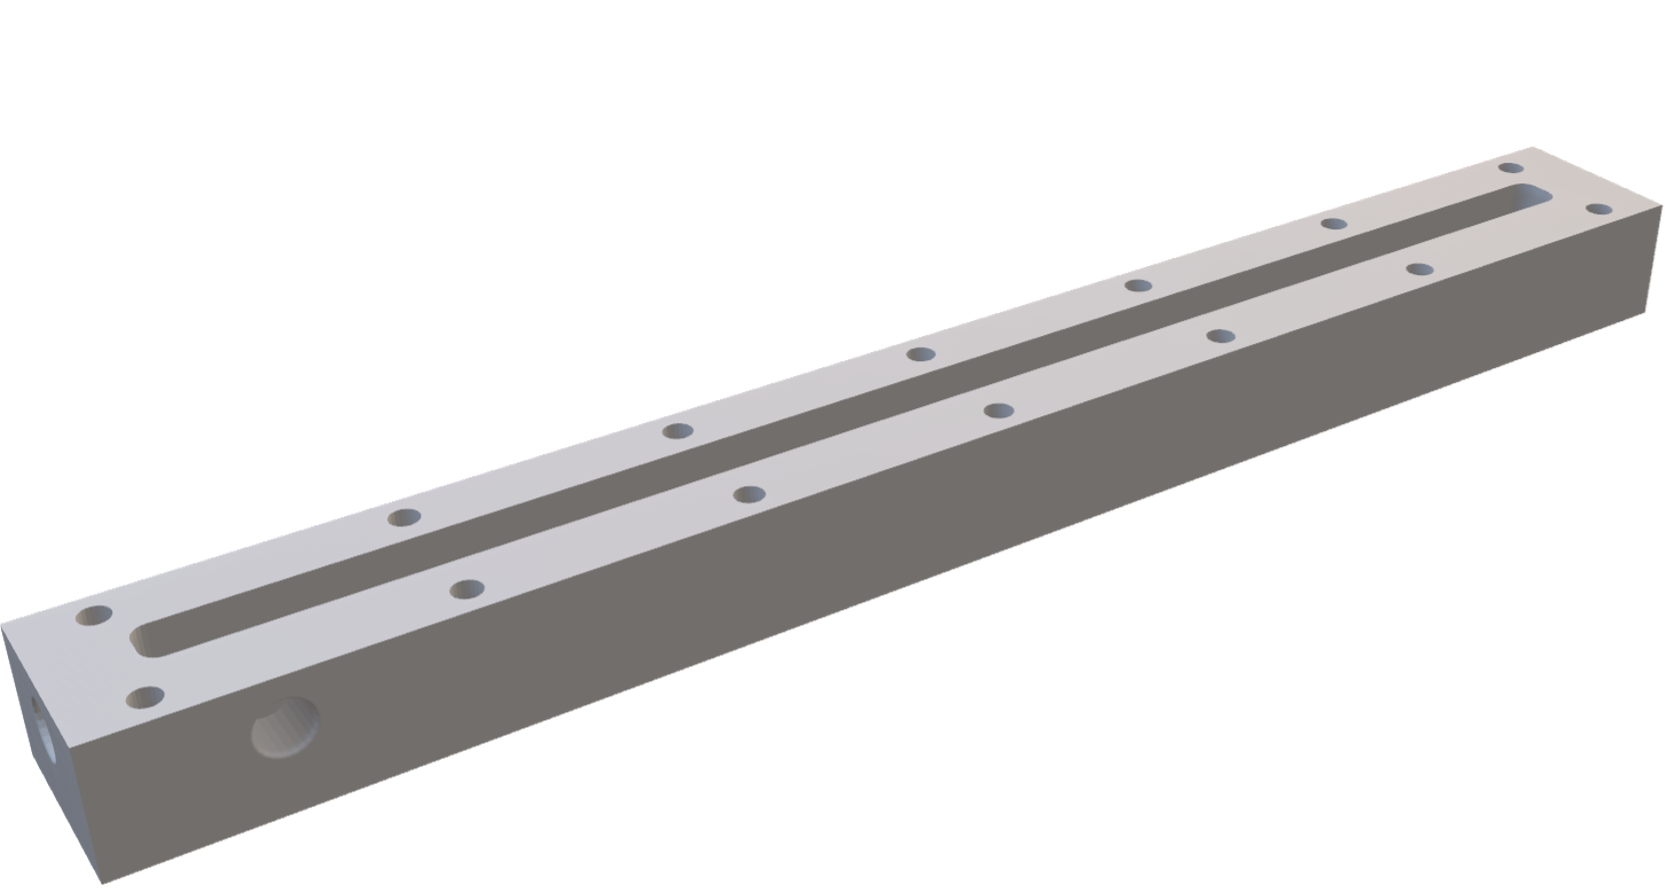
\includegraphics[width=0.5\textwidth]{figures/flowcellCAD.png}
\end{center} 

The viscosity ratio of each experiment will be adjusted by altering the fluid used for the droplets; the $Ca$ and $Re$ depend both on the velocity of the flow, as well as the properties of the chosen fluid. The geometry of the channel will be adjusted using an acrylic insert which fits inside of the base channel. As long as the fluid parameters have a low $Re$ ($Re < 1$), the macroscopic scale of the experiment will not affect the ability of the setup to model microfluidic phenomena. 

Experimental data is collected in the form of videos of the droplet moving through the channel. These videos are analyzed using computer-vision techniques (such as edge detection, optical flow, and background subtraction). To aid in isolating the visual data of just the droplets from the videos, we are dyeing the fluids using two dyes (food coloring for the water/glycerol mixture, and an oil-soluble dye for the PDMS droplets). The videos we have collected until now have been analyzed using the FIJI/ImageJ image processing packages, but the software takes a long time to perform the analysis and is very memory-intensive. To overcome these issues, I am working on in-house software implementing the same computer-vision processing using Python and the \verb|openCV| libary. Currently the software is able to isolate the droplet from the video, and track the centroid but several additions need to be implemented to improve the accuracy of the data. Namely:
\begin{enumerate}
    \item Background subtraction (currently the droplet is isolated using hard-coded parameters)
    \item Camera lens distortion correction
    \item Angle adjustment of each frame of the video based on the outline of the channel (since it is difficult to record videos from the exact same position every time)
    \item Non-dimensional trajectory tracking (currently it is pixel-based)
    \item Taylor Deformation tracking over time (quantitatively measuring the deformation of the droplets)
\end{enumerate}

For \textbf{Aim 2}, we will be running Fortran Boundary-Integral simulations with the same parameters as our experimental fluid systems. Fluid viscosities, densities, $Ca$, and $Re$ must be experimentally determined for each set of conditions run for Aim 1, and the channel geometry is set by the design of the insert. After these parameters are determined, they can be inputted into code previously written by the Davis Group. These simulations are somewhat computationally intensive, therefore the CU Summit supercomputer will be used to run them. 

For \textbf{Aim 3} (a desirable, but not strictly necessary deliverable) I have reached out to Professor Xiaoyun ``Sean" Ding of the Mechanical Engineering department here at CU, as his group works with scale microfluidic chips, and his lab has the manufacturing capabilities to make chips in-house. My intention was to extend this project to also analyze the microfluidic-scale version of the same setup. Doing so would serve as a validation of not only the Boundary-Integral simulations, but also the accuracy of the macroscopic flow-cell to represent microfluidic phenomena. Professor Ding has agreed to allow me to work with his lab under the condition that I am supervised by one of his Ph.D. students or postdocs. Currently, his group is too busy to accommodate any of my proposed experiments, but I will continue to communicate with them in order to try and facilitate these experiments.

\printbibliography

\end{document}